% ======================================================================
%  DROP-IN for au_five_hypotheses: figure + subsection 2.4
%  Requires \usepackage{graphicx}.  Place fig_star_dense.pdf beside the .tex.
%  Insert after Section 2.2 (Redundancy is distributed).
% ======================================================================
\begin{figure}[t]
  \centering
  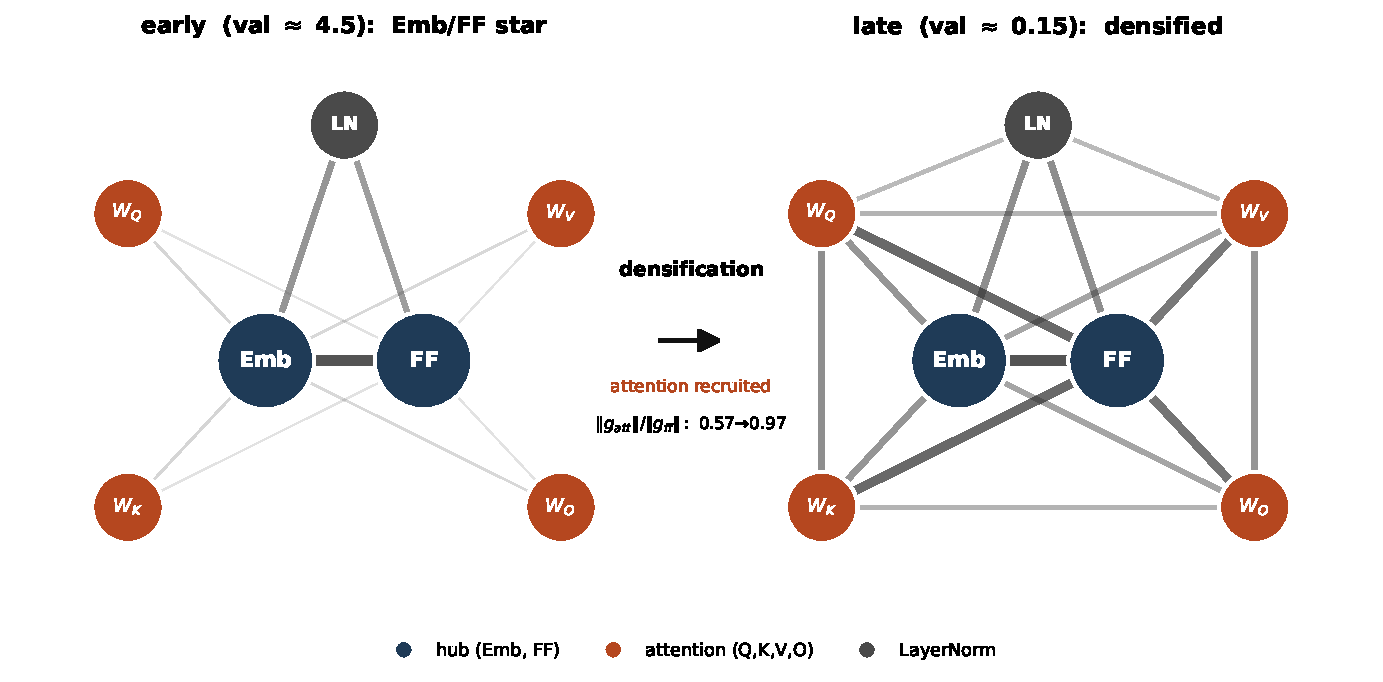
\includegraphics[width=\textwidth]{fig_star_dense.pdf}
  \caption{The block-to-block gradient-coupling graph across the descent.
    \emph{Left}: early ($\mathrm{val}\approx4.5$) the graph is an Emb/FF star---
    the embedding and feed-forward blocks form a hub, attention is peripheral
    (perturbing $W_Q,W_K,W_V,W_O$ does not move FF's gradient).
    \emph{Right}: late ($\mathrm{val}\approx0.15$), on a corpus that recruits
    attention, the graph densifies as induction structure forms. Edge width is
    coupling strength $I_{ab}$; hub in blue, attention in orange. The star is why
    a coherent block is freezable early and not late.}
  \label{fig:stardense}
\end{figure}

\subsection{The interaction graph densifies; freezability is a function of phase}
\label{sec:densify}
The block-to-block gradient coupling
\[
  I_{ab} \;=\; \bigl\| \partial^{2}\mathcal{L}/\partial\theta_{a}\,\partial\theta_{b} \bigr\|,
\]
estimated by Hessian--vector products (no basis, no SVD, so none of the
degeneracy of \S1 enters), is not static across the descent. Early it is a
\emph{star}: the embedding and feed-forward blocks form a hub
($I_{\mathrm{Emb},\mathrm{FF}}$ large from step~$0$), while attention is
peripheral. On corpora that recruit attention, the graph later
\emph{densifies}: the attention--FF coupling and the gradient-norm ratio
$\lVert g_{\mathrm{att}}\rVert/\lVert g_{\mathrm{ff}}\rVert$ rise monotonically
($0.57\!\to\!0.97$ over $\mathrm{val}\,4.5\!\to\!0.08$ on the looped corpus, two
runs), as induction structure forms (Fig.~\ref{fig:stardense}).

This recasts the freezing result of \S2.2 as \emph{phase-dependent}. Freezing
all of attention converges, but at $3.5\times$ the step count ($390$ vs.\ $110$;
Table~4): the cost is precisely the edges the densification would have built.
The star is why a coherent block can be frozen early and cannot be frozen late---
by the dense phase every block sits in the communication graph, and severing any
one severs edges the descent is still using. Densification is thus the process by
which the network reaches the distributed, block-agnostic endpoint of
Theorem~2.1 and \S2.2: it starts with structure (a hub) and ends with none.

\paragraph{The prediction, and the null we ran.} Densification is not a law of
transformer training; it is contingent on the task using attention. On a
non-memorising Markov source (per-symbol entropy floor $\ln k$), the graph does
\emph{not} densify: $\lVert g_{\mathrm{att}}\rVert/\lVert g_{\mathrm{ff}}\rVert$
\emph{falls} to $0.04$, and attention stays freely freezable throughout. The
star is the invariant; the dense phase is the contingency, and which one obtains
is a property of the corpus, not of the architecture.

\paragraph{The null we did not run, stated plainly.} In keeping with the rest of
this paper: we have \emph{not} tested $I_{ab}$ against an untrained-weight null,
as we did for $E$ (\S1.2). The Emb/FF star may already be present at
initialisation---a function of architecture shape, like $E$ itself---in which
case only the densification, and not the star, is a fact about learning. The
causal evidence for block-irreducibility remains the freezing table; the graph
is the mechanism that table suggests, not an independent proof. Fig.~\ref{fig:stardense}
should be read as an illustration of the freezing data, not as a sixth invariant
awaiting its own control.
